\documentclass[11pt,letterpaper]{article}
\usepackage[margin=0.9in]{geometry}
\usepackage[T1]{fontenc}
\usepackage{lmodern,graphicx,booktabs,tabularx,amsmath,natbib,caption,float,placeins}
\usepackage[hidelinks]{hyperref}
\usepackage{microtype}
\captionsetup{font=small,labelfont=bf}
\setlength{\parskip}{4pt}
\setlength{\parindent}{0pt}
\renewcommand{\arraystretch}{1.12}
\bibliographystyle{plainnat}
\title{Evidence Benefits and Repeated Classification Losses in LLM Fact Verification}
\author{Chimdumebi Mitchell Nebolisa \and Jessica Udry}
\date{October 17, 2026}
\begin{document}
\maketitle
\begin{abstract}
% P:ABS1
Adding evidence and restricting a classifier to that evidence are different input changes. We separate them in a repeated evaluation of two related large language models on 10,000 balanced binary FEVER records. In the primary first pass, adding selected evidence with the classification instruction fixed raises accuracy from 88.58\% to 96.17\% for GPT-5.4 and from 84.90\% to 95.45\% for GPT-5.4-mini. Gains are 7.59 and 10.55 percentage points, with descriptive cluster-bootstrap 95\% intervals of 7.01--8.19 and 9.87--11.26. Rescues outnumber regressions, although 98 and 145 first-pass classifications regress. Across three repetitions, matched losses exceed identical-prompt directional loss: a correct classification becoming incorrect across fresh calls using the same prompt, and 186 model--claim cases regress every time across 160 distinct claims. An exploratory, unblinded AI analysis of 465 selected cases compares visible features across losses, rescues, and successful outcomes; worked examples distinguish prediction/reference disagreement from unresolved evidence interpretation. The study shows how controlled input contrasts and repeated calls complement aggregate accuracy on this fixed slice during the recorded collection period and under the stated model configurations.
\end{abstract}

\section{Introduction}\label{sec:intro}
% P:I1
A large language model (LLM) can classify a factual claim from the claim alone or from a claim accompanied by source text. In evidence-based fact verification, the task is to assess whether a claim is supported or refuted. Supplying evidence makes the relevant material inspectable, while a benchmark reference label provides a common scoring rule. FEVER supplies claims, labels, and annotated Wikipedia evidence, allowing these components to be compared in a fixed evaluation \citep{thorne-etal-2018-fever,guo-etal-2022-survey}.

% P:I2
Accuracy alone cannot show whether adding evidence preserves previously correct decisions; paired outcomes and repeated calls reveal losses that the overall improvement conceals. Counting those losses alone also leaves an attribution problem. A comparison that adds evidence and changes the instruction simultaneously mixes two input changes. A single observed change lacks a reference for how often the same classifier changes under an identical prompt. Separating these comparisons is necessary to describe what evidence addition contributes beyond a net accuracy difference.

% P:I3
The present experiment holds the classification instruction fixed when moving from claim-only A to evidence-supplied B, then separately adds an evidence-only restriction in C. Three fresh calls under each condition provide an observed identical-prompt comparison for the matched between-condition losses. A \emph{regression} is correct-to-incorrect against the frozen benchmark label, and a \emph{rescue} is the reverse. These are scoring transitions: movement away from the reference does not by itself establish factual deterioration.

% P:I4
The contribution is a joint empirical account of input differences and repeated classification behavior. The A-to-B contrast measures evidence addition under the same task instruction; B-to-C measures the further instruction restriction. Comparing matched losses with identical-prompt directional loss places them against an observed repeat baseline, while reporting recurring losses alongside rescues shows which losses persist across the recorded calls despite the aggregate benefit. Selected claim--evidence examples then clarify what those scoring transitions can mean. This design describes behavior within the tested records, recorded collection period, and stated model configurations; it does not propose a mitigation method or identify an internal causal mechanism.

\section{Related Work}\label{sec:related}
\subsection{Evidence-based verification}
% P:RW1
Evidence-based verification links a claim to material that can support or refute it. FEVER formalizes this task using Wikipedia claims and annotated evidence, while the verification survey distinguishes evidence retrieval from the subsequent assessment of veracity \citep{thorne-etal-2018-fever,guo-etal-2022-survey}. These components create different evaluation questions: whether relevant material is found, and how a classifier responds when particular material is supplied.

% P:RW2
Correct classification need not establish the intended use of evidence. \citet{schuster-etal-2019-towards} show that biases in fact-verification claims can support prediction without the intended evidential reasoning. Claim-only accuracy can therefore provide a behavioral baseline, but does not establish possession of the relevant factual knowledge. Likewise, accuracy with evidence does not identify a particular reasoning process. Aggregate scores leave open which individual classifications are preserved or changed when evidence is supplied.

\subsection{Evidence-related prediction changes}
% P:RW3
Contrastive evidence tests whether classifications respond to relevant changes in the supplied text. Vitamin C pairs claims with closely related evidence that changes the appropriate verification outcome \citep{schuster-etal-2021-get}. In that setting, evidence sensitivity can require a changed predicted label. This differs from asking whether supplying a fixed designated passage preserves a classification that already agrees with a fixed benchmark reference.

% P:RW4
Related work also examines conflicts between stored and supplied information and robustness to input changes. \citet{longpre-etal-2021-entity} study entity-based knowledge conflicts in question answering. FactEval studies word- and character-level perturbations in fact verification \citep{mamta-cocarascu-2025-facteval}. These interventions establish distinct settings for studying changes in returned outputs. They leave open how losses under evidence addition with the instruction fixed compare with variation across fresh calls using an identical prompt.

\subsection{Evidence interpretation and automated assessment}
% P:RW5
Evidence insufficiency means that the supplied material does not settle a relevant support or refutation judgment; it is distinct from a classifier's failure to decide. \citet{atanasova-etal-2022-fact} examine recognition of insufficiency after information is removed from evidence. AmbiFC represents ambiguous claims through competing interpretations and annotator disagreement \citep{glockner-etal-2024-ambifc}. These distinctions matter when interpreting a scored regression: the selected text can omit a necessary fact, permit more than one reading, or appear to conflict with the reference. An automated text review can flag those possibilities without validating a replacement label.

% P:RW6
Automated judgments themselves require qualification. \citet{chen-etal-2024-humans} examine judgment bias in LLM evaluation, supporting scrutiny of the evaluator rather than treating its output as ground truth. Automated interpretation of claim--evidence relations therefore requires disclosure of the evaluator and review procedure, alongside a distinction between interpretive flags and benchmark scoring.

% P:RW7
The present experiment addresses these evaluation questions by supplying a fixed designated evidence set under an unchanged classification instruction, then testing an additional evidence-only restriction separately. Paired outcomes show which classifications improve or regress, and repeated identical-prompt calls provide an observed directional-loss comparison. An exploratory selected-case analysis examines visible claim--evidence features and interpretation concerns; its unblinded AI judgments remain separate from the frozen benchmark scores. Earlier Evidex judge-family analyses concern a different cohort and procedure, documented in Supplement S4.

\section{Methodology}\label{sec:methods}
\subsection{Controlled input comparison and data flow}
% P:M1
The workflow begins with fixed claims, reference labels, and selected evidence. Each model classifies every claim separately under A, B, and C. A-to-B changes the evidence content while holding the instruction fixed; B-to-C changes only the evidence-only phrase. Each repetition is a fresh stateless request, rather than another choice returned by one request. Saved raw responses are parsed under the fixed rule and compared with the unchanged reference. The resulting matched outcomes feed the quantitative summaries and a separately selected exploratory case analysis (Figure~\ref{fig:workflow}). Coding never feeds back into benchmark scoring.

\begin{figure}[H]\centering
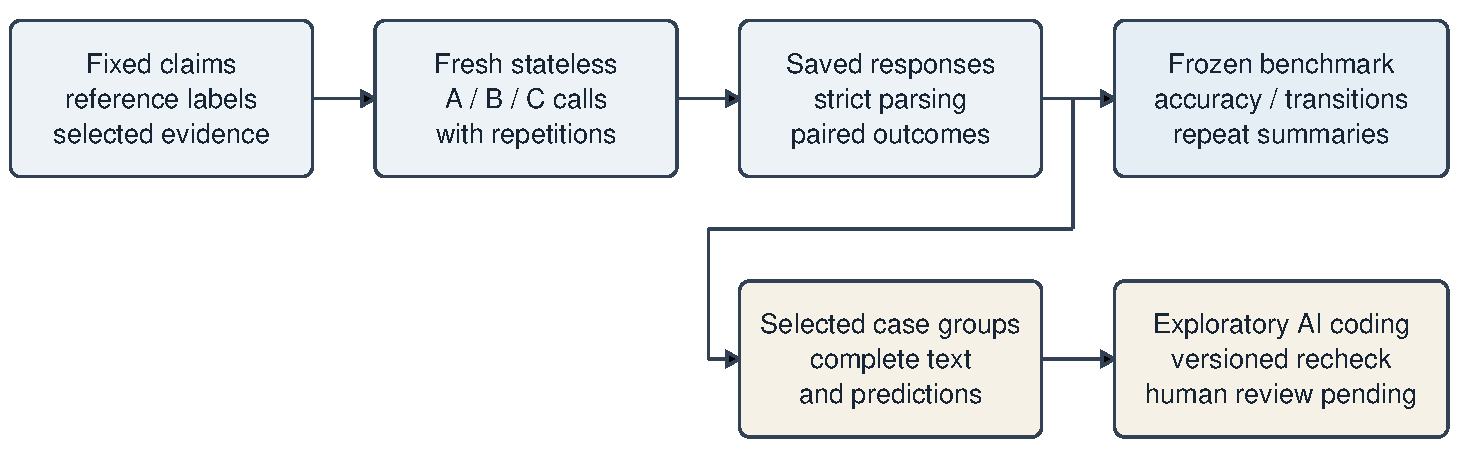
\includegraphics[width=\linewidth]{figures/workflow.pdf}
\caption{Workflow for paired classification and subsequent exploratory case analysis. Arrows show data flow and selection, not causal explanations. Repeated A/B/C calls feed frozen benchmark summaries; selected claim--evidence cases feed AI coding and its documented recheck. Coding does not alter reference labels or benchmark outcomes.}\label{fig:workflow}
\end{figure}

\subsection{Paired outcomes}
% P:M2
For a fixed model, claim, and matched repetition, each contrast has four mutually exclusive outcomes: \emph{stayed correct}, \emph{rescue} (wrong to correct), \emph{regression} (correct to wrong), and \emph{stayed wrong}. They partition the assigned pairs. Left-condition accuracy counts stayed-correct cases plus regressions; right-condition accuracy counts stayed-correct cases plus rescues. Consequently, the accuracy difference equals rescues minus regressions divided by the assigned pair count. The stayed-correct fraction alone is neither condition's accuracy. The same definitions apply to A-to-B, B-to-C, and the combined A-to-C contrast.

\subsection{Repetitions and the variation baseline}\label{sec:repeat-method}
% P:M3
Repeated summaries first reduce outcomes within each claim, then aggregate across claims. They do not treat repeated calls as new independent claim observations. Let $c_{imXr}$ indicate whether model $m$ classifies claim $i$ correctly in condition $X$, repetition $r$, and let $K$ be the assigned number of repetitions. Matched between-condition loss and ordered identical-left-condition loss are
\begin{align}
L^{X\to Y}_{im}&=K^{-1}\sum_r c_{imXr}(1-c_{imYr}),\\
L^{X\to X}_{im}&=[K(K-1)]^{-1}\sum_{r\ne s}c_{imXr}(1-c_{imXs}).
\end{align}
% P:M4
Their difference is the per-claim excess loss relative to observed directional variation under the left prompt. Label disagreement instead counts unequal outputs over unordered pairs. With complete binary outputs, its rate is twice the ordered correct-to-wrong rate: each unequal unordered pair contributes one loss among its two orderings. These are different denominators and quantities. Recurrence records how many matched repetitions have the same outcome, including loss on every recorded repetition; it does not establish a permanent individual property.

\section{Experiments and Results}\label{sec:results}
\subsection{Research questions}
% P:RQ1
The experiment asks: RQ1, how do aggregate accuracy and paired gains and losses differ when selected evidence is added and when the instruction is subsequently restricted? RQ2, how do those losses compare with identical-prompt variation, and which recur over the recorded repetitions? RQ3, what observable claim--evidence features and interpretation concerns accompany selected regressions and comparison outcomes? The first-pass contrasts answer RQ1; repeated summaries answer RQ2; the explicitly exploratory case analysis addresses RQ3 without identifying internal causes.

\subsection{Data, execution, and analysis configuration}\label{sec:setup}
% P:X1
The present experiment reuses a fixed FEVER development slice of 10,000 records: 5,000 Supported and 5,000 Refuted, excluding Not Enough Info. Each input retains its previously selected annotated evidence and unchanged sentence text. A targeted comparison with the \href{https://fever.ai/download/fever/shared_task_dev.jsonl}{official FEVER development release} matched all 10,000 claim texts, reference labels, and selected evidence-pointer sets, using the preparation's existing Unicode NFC title normalization (Supplement S5). This establishes release correspondence, not factual correctness of every annotation. Evidence is supplied directly; ``selected gold evidence'' does not imply retrieval or guaranteed sufficiency under every interpretation.

% P:X2
Requests used \texttt{gpt-5.4} and \texttt{gpt-5.4-mini}. The corresponding returned identifiers were \texttt{gpt-\allowbreak{}5.4-\allowbreak{}2026-\allowbreak{}03-\allowbreak{}05} and \texttt{gpt-\allowbreak{}5.4-\allowbreak{}mini-\allowbreak{}2026-\allowbreak{}03-\allowbreak{}17}. Recorded provider creation times span October 17, 2026, 00:31--13:41 UTC. Three fresh stateless calls per model, claim, and condition yield $10{,}000\times2\times3\times3=180{,}000$ responses. Temperature was zero, with no prior conversation, retrieval, or tools. The joint schedule was shuffled across models, claims, conditions, and repetition indices. Table~\ref{tab:conditions} defines the input contrasts; Appendix~\ref{app:messages} gives exact messages and settings.

@@TABLE_CONDITIONS@@

% P:X3
The frozen parser accepts one valid Supported or Refuted label under strict returned-model, choice, stop, and refusal checks. All 180,000 planned outcomes were valid, with zero failed, invalid, uncertain, missing, or detected duplicate request-bearing submissions. Recording retained requests, raw responses, parsed labels, and usage. Collection resumed after a database interruption without changing the scientific configuration; the execution and recording details are in Supplement S1.

% P:S1
Repetition 1 and the A-to-B and B-to-C contrasts were designated primary before collection; A-to-C is secondary. ``First pass'' names that prespecified index, not chronological finishing order. All-three summaries include repetition 1. Descriptive 95\% intervals use the frozen 2,000-draw bootstrap of 9,855 casefolded, whitespace-normalized claim-text clusters, seed 20261016. Repetitions are reduced within claim before resampling, with shared cluster weights across models, conditions, repetitions, and labels and fixed observed label-stratum proportions. Thus calls are not treated as independent claims. Supplement S2 gives the complete resampling rules and denominators.

% P:T1
The exploratory case sample includes every all-three A-to-B regression (186 model--claim cases across 160 IDs), every all-three B-to-C regression separately (59 cases across 58 IDs), and capped samples of A-to-B rescues, stayed-wrong cases, stayed-correct cases, and mixed-repetition regressions. It contains 465 cases across 416 distinct claims. Seeded sampling and the codebook are documented in Supplement S3. Multiple visible feature labels are allowed; a separate assessment records support, apparent conflict, insufficiency, or ambiguity relative to the frozen reference.

% P:T2
The same unblinded AI assistant coded the cases and performed a subsequent review covering 230 of the 416 claims; 186 did not receive second review. No independent coding or human validation was performed. Reference-conflict assessments remain review flags, and neither coding nor rechecking changes benchmark labels or scores. Coverage, revisions, and complete case records are retained in Supplement S3.

\subsection{Primary accuracy benefits and paired losses}\label{sec:primary}
% P:B1
Adding selected evidence improves first-pass benchmark accuracy for both models while leaving a smaller set of paired losses. GPT-5.4 rises from 88.58\% in A to 96.17\% in B; mini rises from 84.90\% to 95.45\% (Table~\ref{tab:accuracy}). The corresponding gains are 7.59 percentage points (descriptive 95\% interval 7.01--8.19) and 10.55 points (9.87--11.26). Because A and B use the same instruction, these gains quantify evidence addition under the same classification task.

@@TABLE_ACCURACY@@

% P:B2
Rescues explain the positive net gains, but do not erase regressions (Table~\ref{tab:transitions}). A-to-B produces 857 rescues and 98 regressions for GPT-5.4, and 1,200 rescues and 145 regressions for mini. Thirty-four claim IDs regress for both models, so $98+145-34=209$ distinct records account for 243 model--claim regression observations. The remaining 8,760/285 and 8,345/310 pairs stayed correct/stayed wrong for main/mini. These joint counts distinguish improvement from preservation without treating overlapping model observations as independent claims.

@@TABLE_TRANSITIONS@@

% P:B3
The evidence-only instruction changes much less than evidence addition in the first pass. B-to-C gives a 0.05-point difference for GPT-5.4 (-0.14--0.24) and 0.25 points for mini (0.01--0.51). Its regressions/rescues are 41/46 and 66/91. The small positive lower bound for mini is part of the descriptive interval family, not an isolated confirmatory discovery. Neither these estimates nor intervals containing zero establish equivalence. The secondary A-to-C contrast combines both input changes and is retained separately in Appendix~\ref{app:outcomes}.

\subsection{Repeat variation and recurring losses}\label{sec:variation}
% P:V1
Averaging all three repetitions preserves the large observed evidence benefit while making within-claim variation visible. GPT-5.4's A, B, and C accuracies are respectively 88.61\%, 96.16\%, and 96.18\%; mini's are 84.73\%, 95.52\%, and 95.69\%. A-to-B gains are 7.55 points (6.95--8.14) and 10.79 (10.13--11.44); B-to-C gains are 0.02 (-0.16--0.20) and 0.17 (-0.02--0.37). These summaries contain 30,000 calls per model/condition but only 10,000 claim IDs, and include the primary first pass. They are not an independent replication of it. Full estimates and interval endpoints remain in the frozen output and supplementary result tables.

@@TABLE_REPEAT@@

% P:V2
Identical messages do not always yield identical labels at temperature zero (Table~\ref{tab:variability}). Unordered-pair disagreement is 0.667\%/0.153\%/0.193\% in A/B/C for GPT-5.4 and 2.333\%/0.713\%/0.653\% for mini. The ordered directional loss baseline is half each rate for these complete binary outputs, as defined in Section~\ref{sec:repeat-method}. Matched between-condition losses exceed that baseline in both primary contrasts (Table~\ref{tab:excess}). The A-to-B excess is 0.670 percentage points (0.481--0.871) for main and 0.253 (0.019--0.490) for mini; B-to-C excesses are 0.387 (0.267--0.508) and 0.310 (0.183--0.440). The subtraction describes observed loss frequencies under this design, not the fraction of latent permanent or causal failures.

@@TABLE_VARIABILITY@@

@@TABLE_EXCESS@@

% P:V3
Some losses recur in every recorded matched repetition. A-to-B has 87 such GPT-5.4 cases and 99 mini cases, overlapping on 26 IDs: 186 model--claim cases across 160 distinct claims. B-to-C has 32 and 27 cases, overlapping on one ID: 59 cases across 58 claims. Across any of the repetitions, A-to-B regression appears in 301 model--claim cases across 255 IDs; the all-three cohort is a subset. The complete four-outcome count vector for every model--claim--contrast is retained, so mixed rescues, losses, and unchanged outcomes are not collapsed into a stability label. Three observed losses establish finite recurrence, not a permanent individual failure.

\subsection{Exploratory case analysis}\label{sec:cases}
% P:C1
The case analysis distinguishes a visible comparison demand from an explanation of a model's error. Table~\ref{tab:examples} gives four worked examples from existing records. The same negation demand accompanies a recurring regression and a successful rescue. Other rows show why a repeated benchmark loss can leave a text/reference or interpretation question unresolved.

% P:C2
The comparison groups make that distinction concrete. Numerical features occur in 65 of 186 selected recurring A-to-B regression cases and 34 of 60 sampled rescue cases (Table~\ref{tab:features}). A numerical comparison can therefore accompany either outcome; its presence is not sufficient to explain a regression. These counts use selected model--claim--contrast cases, allow overlapping features, and compare an exhaustive recurring-loss group with a capped rescue sample. They describe the selected cases rather than estimate population prevalence or identify a causal mechanism.

@@TABLE_EXAMPLES@@

% P:C3
The interpretation axis serves a different purpose from feature coding. The KGB example flags an explicit tension between the supplied sentence and the reference; the chart-position example preserves competing readings of a numerical statement. Those concerns qualify how a scored loss is described without replacing its reference label. The full assessment table and pending-review cases are provided in Supplement S3.

\subsection{Reproducibility, recovery, and usage}\label{sec:repro}
% P:P1
The \href{https://github.com/ChimdumebiNebolisa/Evidex/tree/3893a57e6f9addadf2b2fcd2d5a4e7251abcb677/replacement_predictor_v1/published/full3-2026-10-17}{pinned results bundle} provides the protocol, source snapshots, frozen analysis, and provenance inventories; individual raw request/response bytes remain in the preserved local archive. Collection finished on October 17, 2026, at 13:42 UTC after database recovery. A later operating-system restart interrupted offline analysis; recovery used the unchanged analysis source and settings, completing at 23:35 UTC. Supplement S1 records the execution chronology, recording checks, usage, and archive access boundaries. The companion supplementary package assembles S1--S5, including later audit and coding records that are separate from the pinned results bundle.

\section{Discussion and Conclusion}\label{sec:discussion}
\subsection{What the comparison establishes}
% P:D1
The results separate the overall value of supplied evidence from preservation of individual benchmark-correct answers. The primary A-to-B gains are substantial, while the joint counts expose smaller paired losses and show how many rescues underlie the improvement. B-to-C changes are much smaller in this experiment, so combining that instruction change with evidence addition would obscure the distinction between them. The repeated comparison adds a reference for interpreting losses: matched between-condition losses exceed the observed directional variation under identical messages. That excess is a descriptive difference between measured rates, not a causal decomposition of error.

% P:D2
Recurrence adds information that a single paired output cannot provide. Losses on all three recorded matches identify a repeat pattern within these calls, even while overall accuracy improves. The selected examples show why such a pattern still needs interpretation: the model can disagree with a clear local relation, follow a sentence that conflicts with the reference, or confront competing numerical readings. Comparing regressions with rescues and successful cases prevents a common textual feature from being treated as an explanation merely because it occurs in a loss.

\subsection{Evaluation and historical interpretation}
% P:D3
For this evaluation, aggregate accuracy, paired transitions, repeated variation, and supplied-text interpretation answer different questions. Reporting them together makes an evidence benefit assessable without hiding losses or treating every benchmark disagreement as factual deterioration. Earlier Evidex predictions, natural language inference diagnostics, and automated judging used a separate historical cohort, including the original 226 claims; they are context rather than additional observations from the present experiment. Supplement S4 preserves their results and methodological qualifications.

\subsection{Limitations}
% P:L1
The balanced binary FEVER slice excludes Not Enough Info, natural label frequencies, and retrieval, so the results concern supplied-text classification rather than deployed fact verification. Training exposure to the claims or Wikipedia source is unknown. Identical claim texts can have different references under different supplied contexts; claim-only A cannot identify a context absent from its input. Text clustering addresses statistical dependence, not that semantic ambiguity. Correspondence with the official release does not independently verify the truth of its labels or every Wikipedia sentence.

% P:L2
The two models are related GPT variants observed during one recorded collection period under the stated model configurations. Snapshot identifiers do not exclude hidden serving changes, and system fingerprints were unreported. Three calls at temperature zero describe finite variation rather than future stability. Bootstrap intervals condition on the recorded outputs and label balance; they do not cover all provider or population uncertainty, and small instruction differences do not establish equivalence.

% P:L3
The taxonomy is an exploratory, outcome-enriched sample with overlapping features, unblinded AI coding, incomplete second review, and no human validation. Its counts cannot estimate population error prevalence or adjudicate true reference errors. Stronger reference-correction claims would require source and human adjudication.

\subsection{Conclusion}
% P:CON1
Adding selected evidence under a fixed instruction improves first-pass reference-label accuracy for both tested models, with rescues exceeding regressions. Separating the instruction contrast, measuring identical-prompt directional loss, and recording finite recurrence provide information that the net gain alone omits. The exploratory cases make the interpretation of those benchmark transitions more specific while preserving unresolved reference and evidence questions. Together, these measurements give a bounded account of evidence benefits and recurring losses on the tested FEVER slice.

\bibliography{references}
\clearpage
\appendix
\section{Exact messages and execution settings}\label{app:messages}
% P:APM1
The following templates use literal line breaks. Braced fields are replaced by the unchanged prepared strings. Every call has one user message; the request body adds only the model identifier and settings described in Section~\ref{sec:setup}. A contains no empty evidence field. The three conditions are not the historical judge-disclosure stages, which used different inputs and labels.
\begin{quote}\small\ttfamily
Classify the claim as Supported or Refuted.\\
Output only one word: Supported or Refuted.\\[4pt]
Claim: \{claim\_text\}
\end{quote}
% P:APM2
Condition B appends \texttt{Evidence: \{gold\_evidence\}} on a new line after the claim. Condition C instead uses the first sentence below, followed by the same one-word output instruction, blank line, claim, and evidence as B.
\begin{quote}\small\ttfamily
Classify the claim as Supported or Refuted based only on the evidence provided.
\end{quote}
% P:APM3
Requests used the direct OpenAI Chat Completions endpoint. The output contract accepts exactly the requested binary label with the frozen minimal normalization and validates raw structure, finish reason, refusal, and returned identity. Plan/job hashes, receipts, raw bytes, parsed results, and usage remain linked. Complete materialized request examples and all scientific settings are in the pinned publication bundle; raw request headers containing credentials were not archived.

% P:APM4
Every request used one user message and no system/developer message, history, retrieval, tools, or appended run identifier. Settings were temperature 0, reasoning effort \texttt{none}, completion cap 32 tokens, $n=1$, non-streaming, storage disabled, and requested service tier \texttt{default}; no API sampling seed varied across calls. The joint schedule used seed 20261016. Returned service tiers were \texttt{default}; system fingerprints were unreported. The original fixed-slice extraction recorded seed 42.

\section{Complete outcome and repetition records}\label{app:outcomes}
% P:APO1
Table~\ref{tab:secondary} reports the secondary A-to-C contrast, which combines evidence addition and the instruction restriction. Its first-pass counts use 10,000 matched pairs per model; all-three changes average within those same 10,000 claims. Supplement S2 retains the complete four-outcome vectors and repetition records.

@@TABLE_SECONDARY@@

% P:APO2
Secondary A-to-C all-three recurrence is 208 model--claim cases across 174 IDs. Across any matched repetition it appears in 320 model--claim cases across 264 IDs. These combine evidence and instruction changes, rather than adding evidence alone. Fresh outcomes within the historically selected cohort are reported separately in the frozen summary; they are not the historical predictors' recorded responses.

\section{Feature counts in the selected cases}\label{app:taxonomy}
% P:APT2
Features describe visible comparison demands: negation (NEG), scope or degree (SCOPE), relations and roles (REL), entities and attribute fillers (ENT), numerical comparison (NUM), semantic readings or granularity (LEX), contextual linkage (CTX), missing warrant in the supplied text (GAP), and material wording or extraction issues (TXT). DIRECT is an ordinary local match or mismatch with no distinctive feature; UNCLEAR retains unresolved coding. Multiple labels may apply, except that DIRECT does not accompany a substantive feature.

@@TABLE_FEATURES@@

% P:APT3
Table~\ref{tab:features} counts selected model--claim--contrast cases, so feature totals can exceed group sizes. Cases can overlap across claim IDs and selection groups. The supplied-text assessment axis, sampling definitions, AI review coverage, and complete case records appear in Supplement S3.

\end{document}
